\begin{figure}[htbp]
    \def\subfigheight{4.5cm}
    \centering
    \begin{subfigure}[t]{.19\textwidth}
        \centering
        %\includesvg[height=\subfigheight]{samples/inverted/samples_1184_0.svg}
        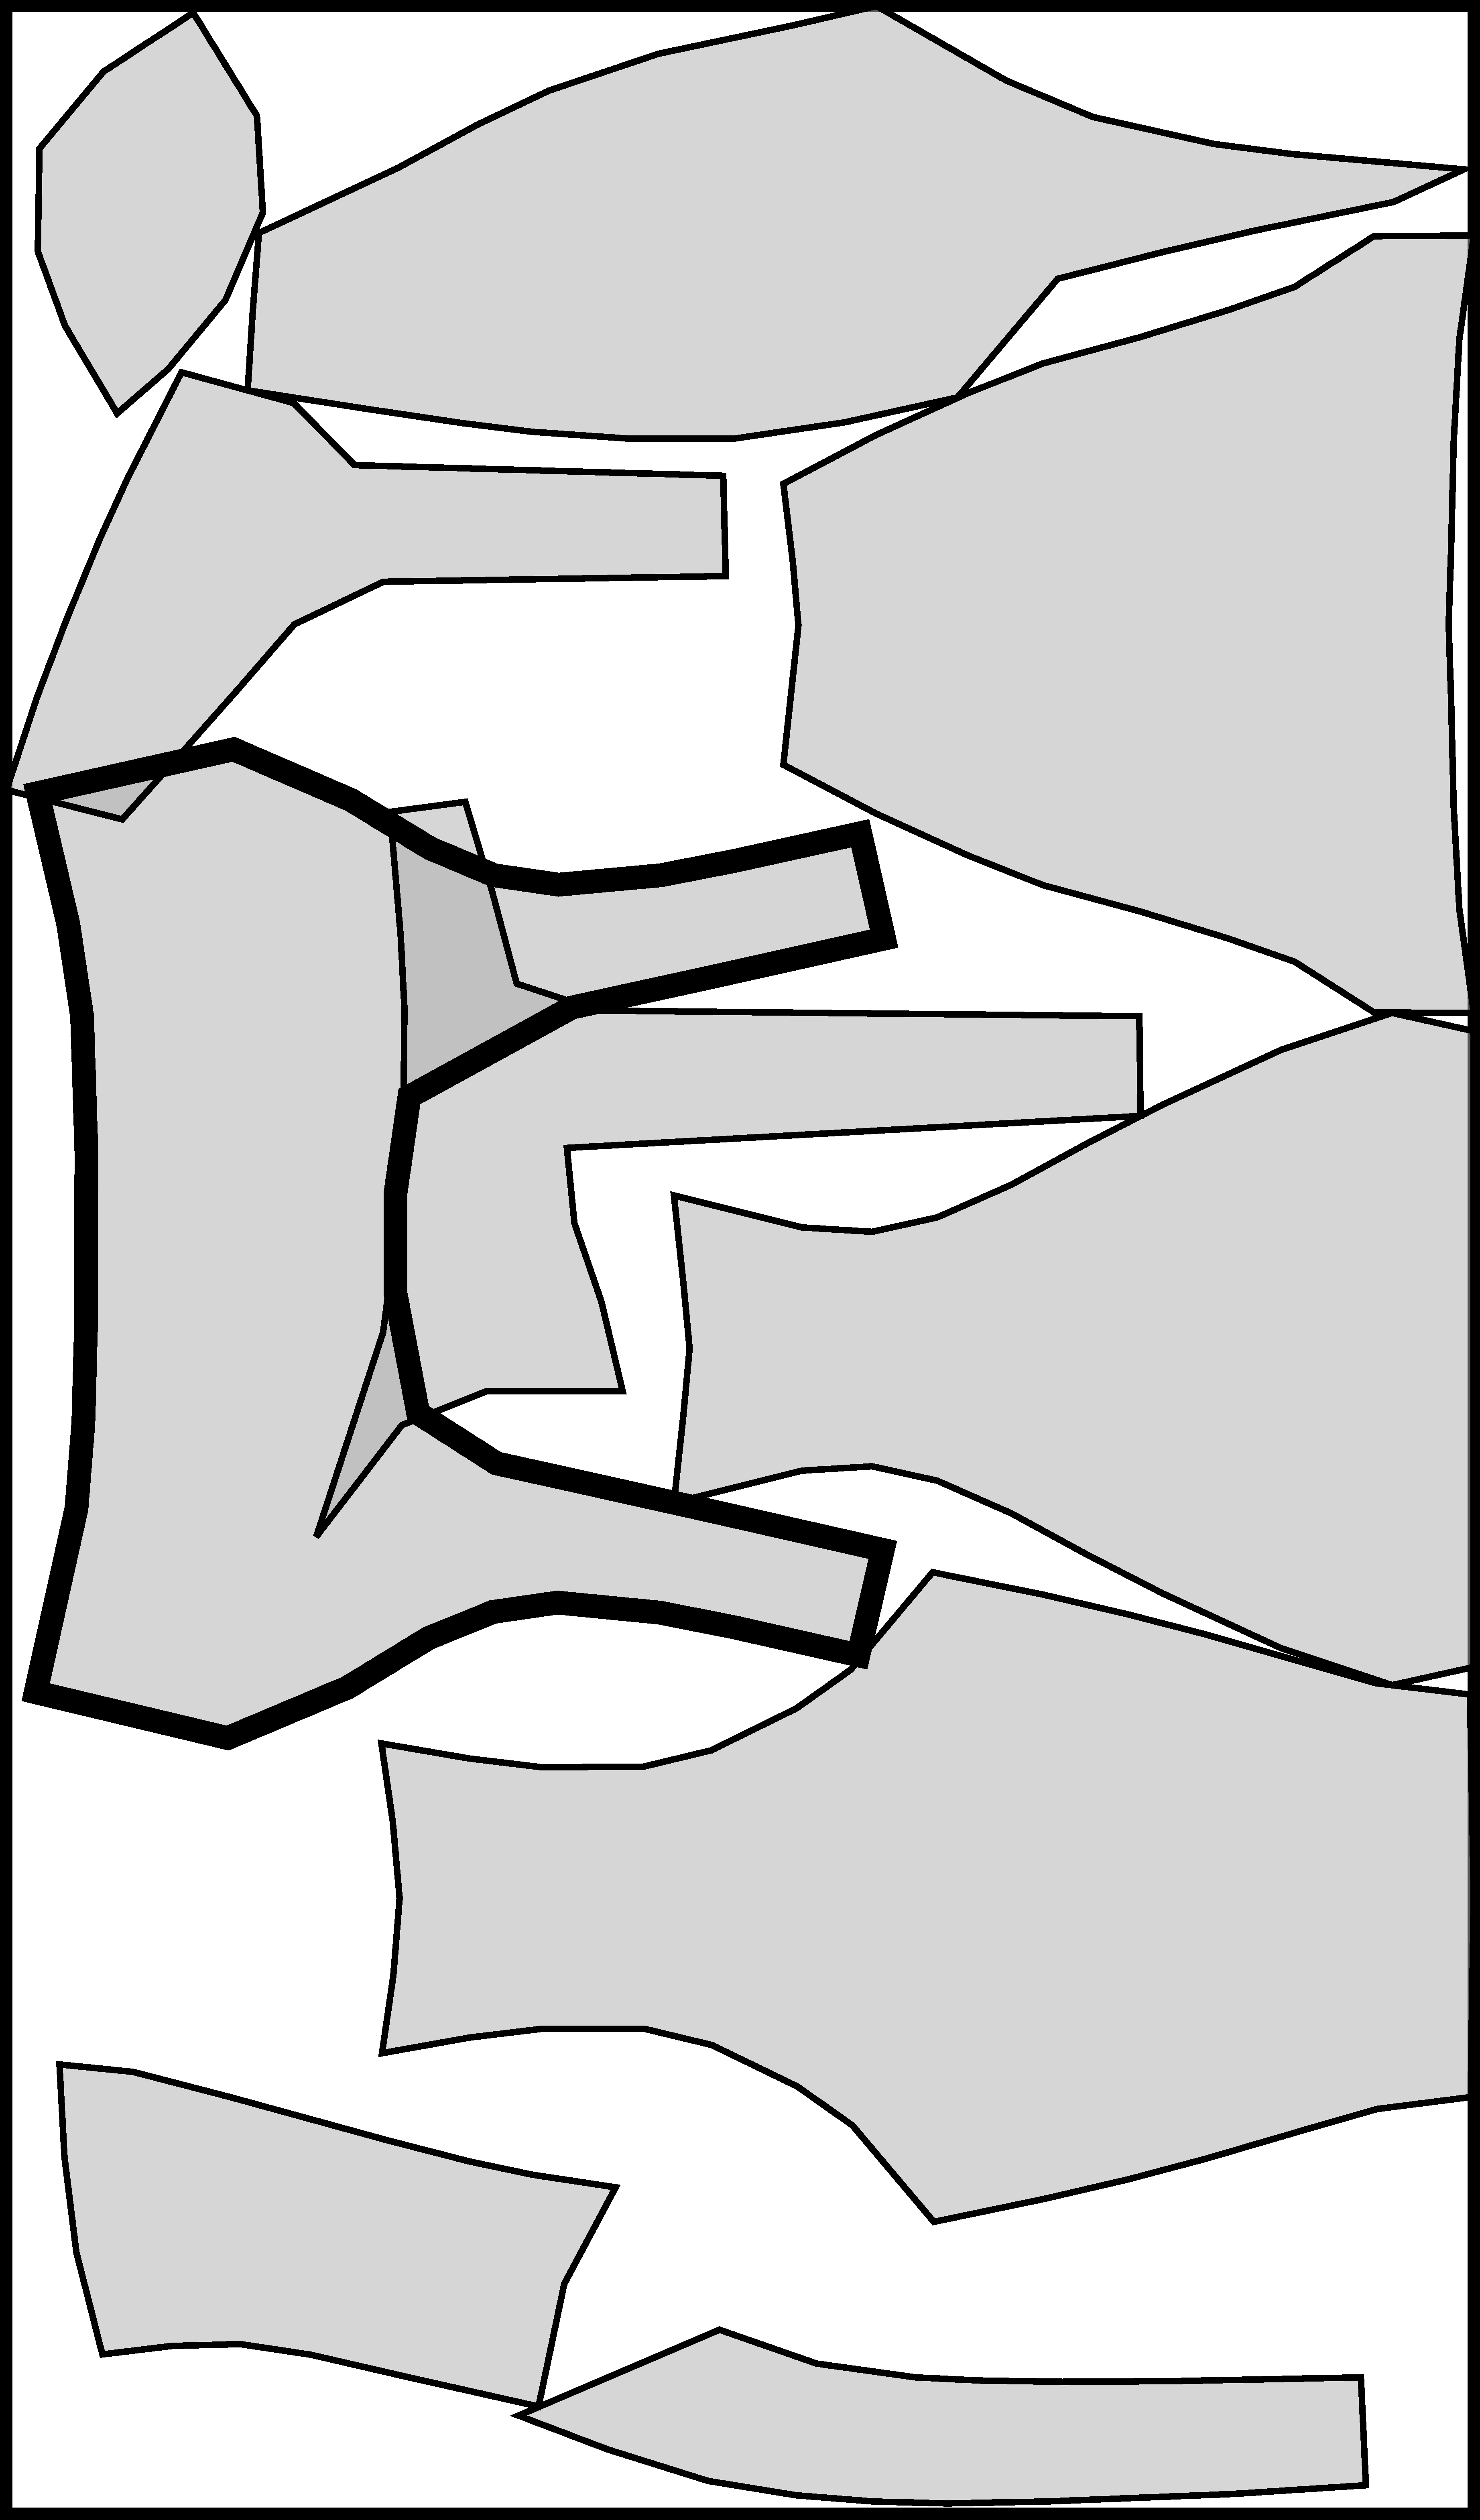
\includegraphics[height=\subfigheight]{samples_1184_0_svg-tex.pdf}
        \caption{Before}
        \label{fig:sampling_before}
    \end{subfigure}
    \begin{subfigure}[t]{.19\textwidth}
        \centering
        %\includesvg[height=\subfigheight]{samples/inverted/samples_1184_1.svg}
        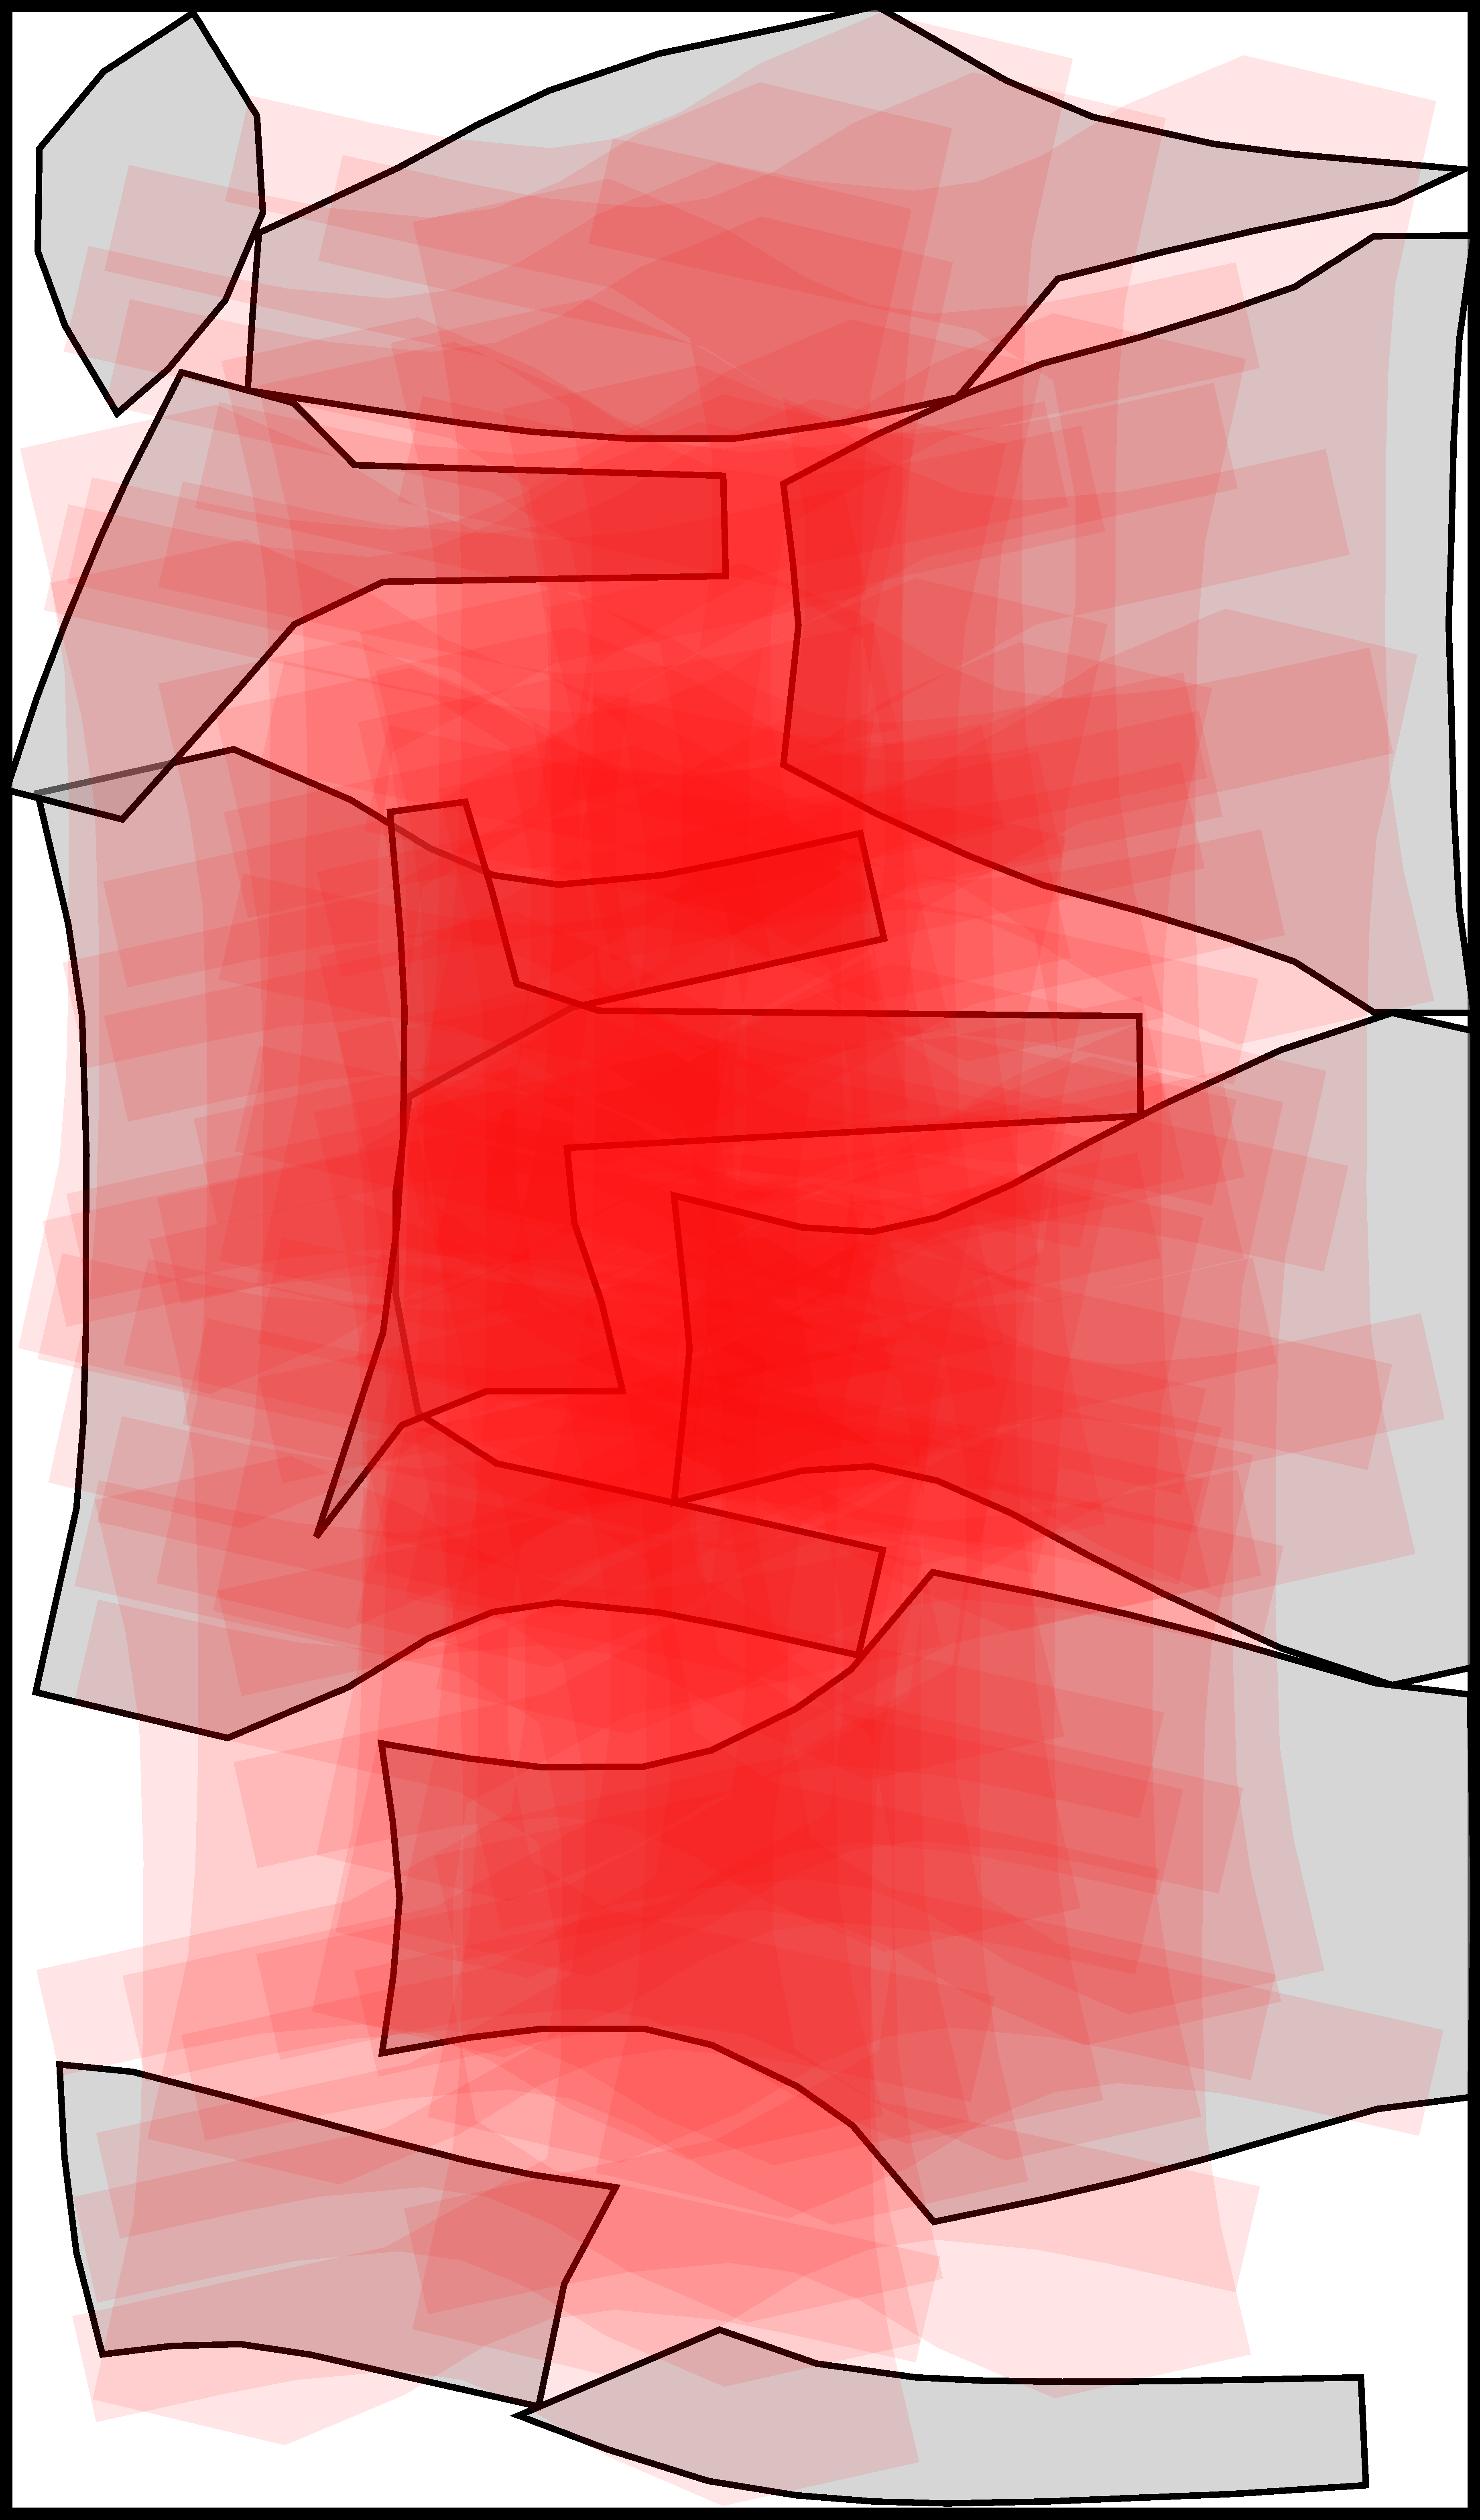
\includegraphics[height=\subfigheight]{samples_1184_1_svg-tex.pdf}
        \caption{Random samples in the strip: $T_{div}$}
        \label{fig:sampling_bin}
    \end{subfigure}
    \begin{subfigure}[t]{.19\textwidth}
        \centering
        %\includesvg[height=\subfigheight]{samples/inverted/samples_1184_2.svg}
        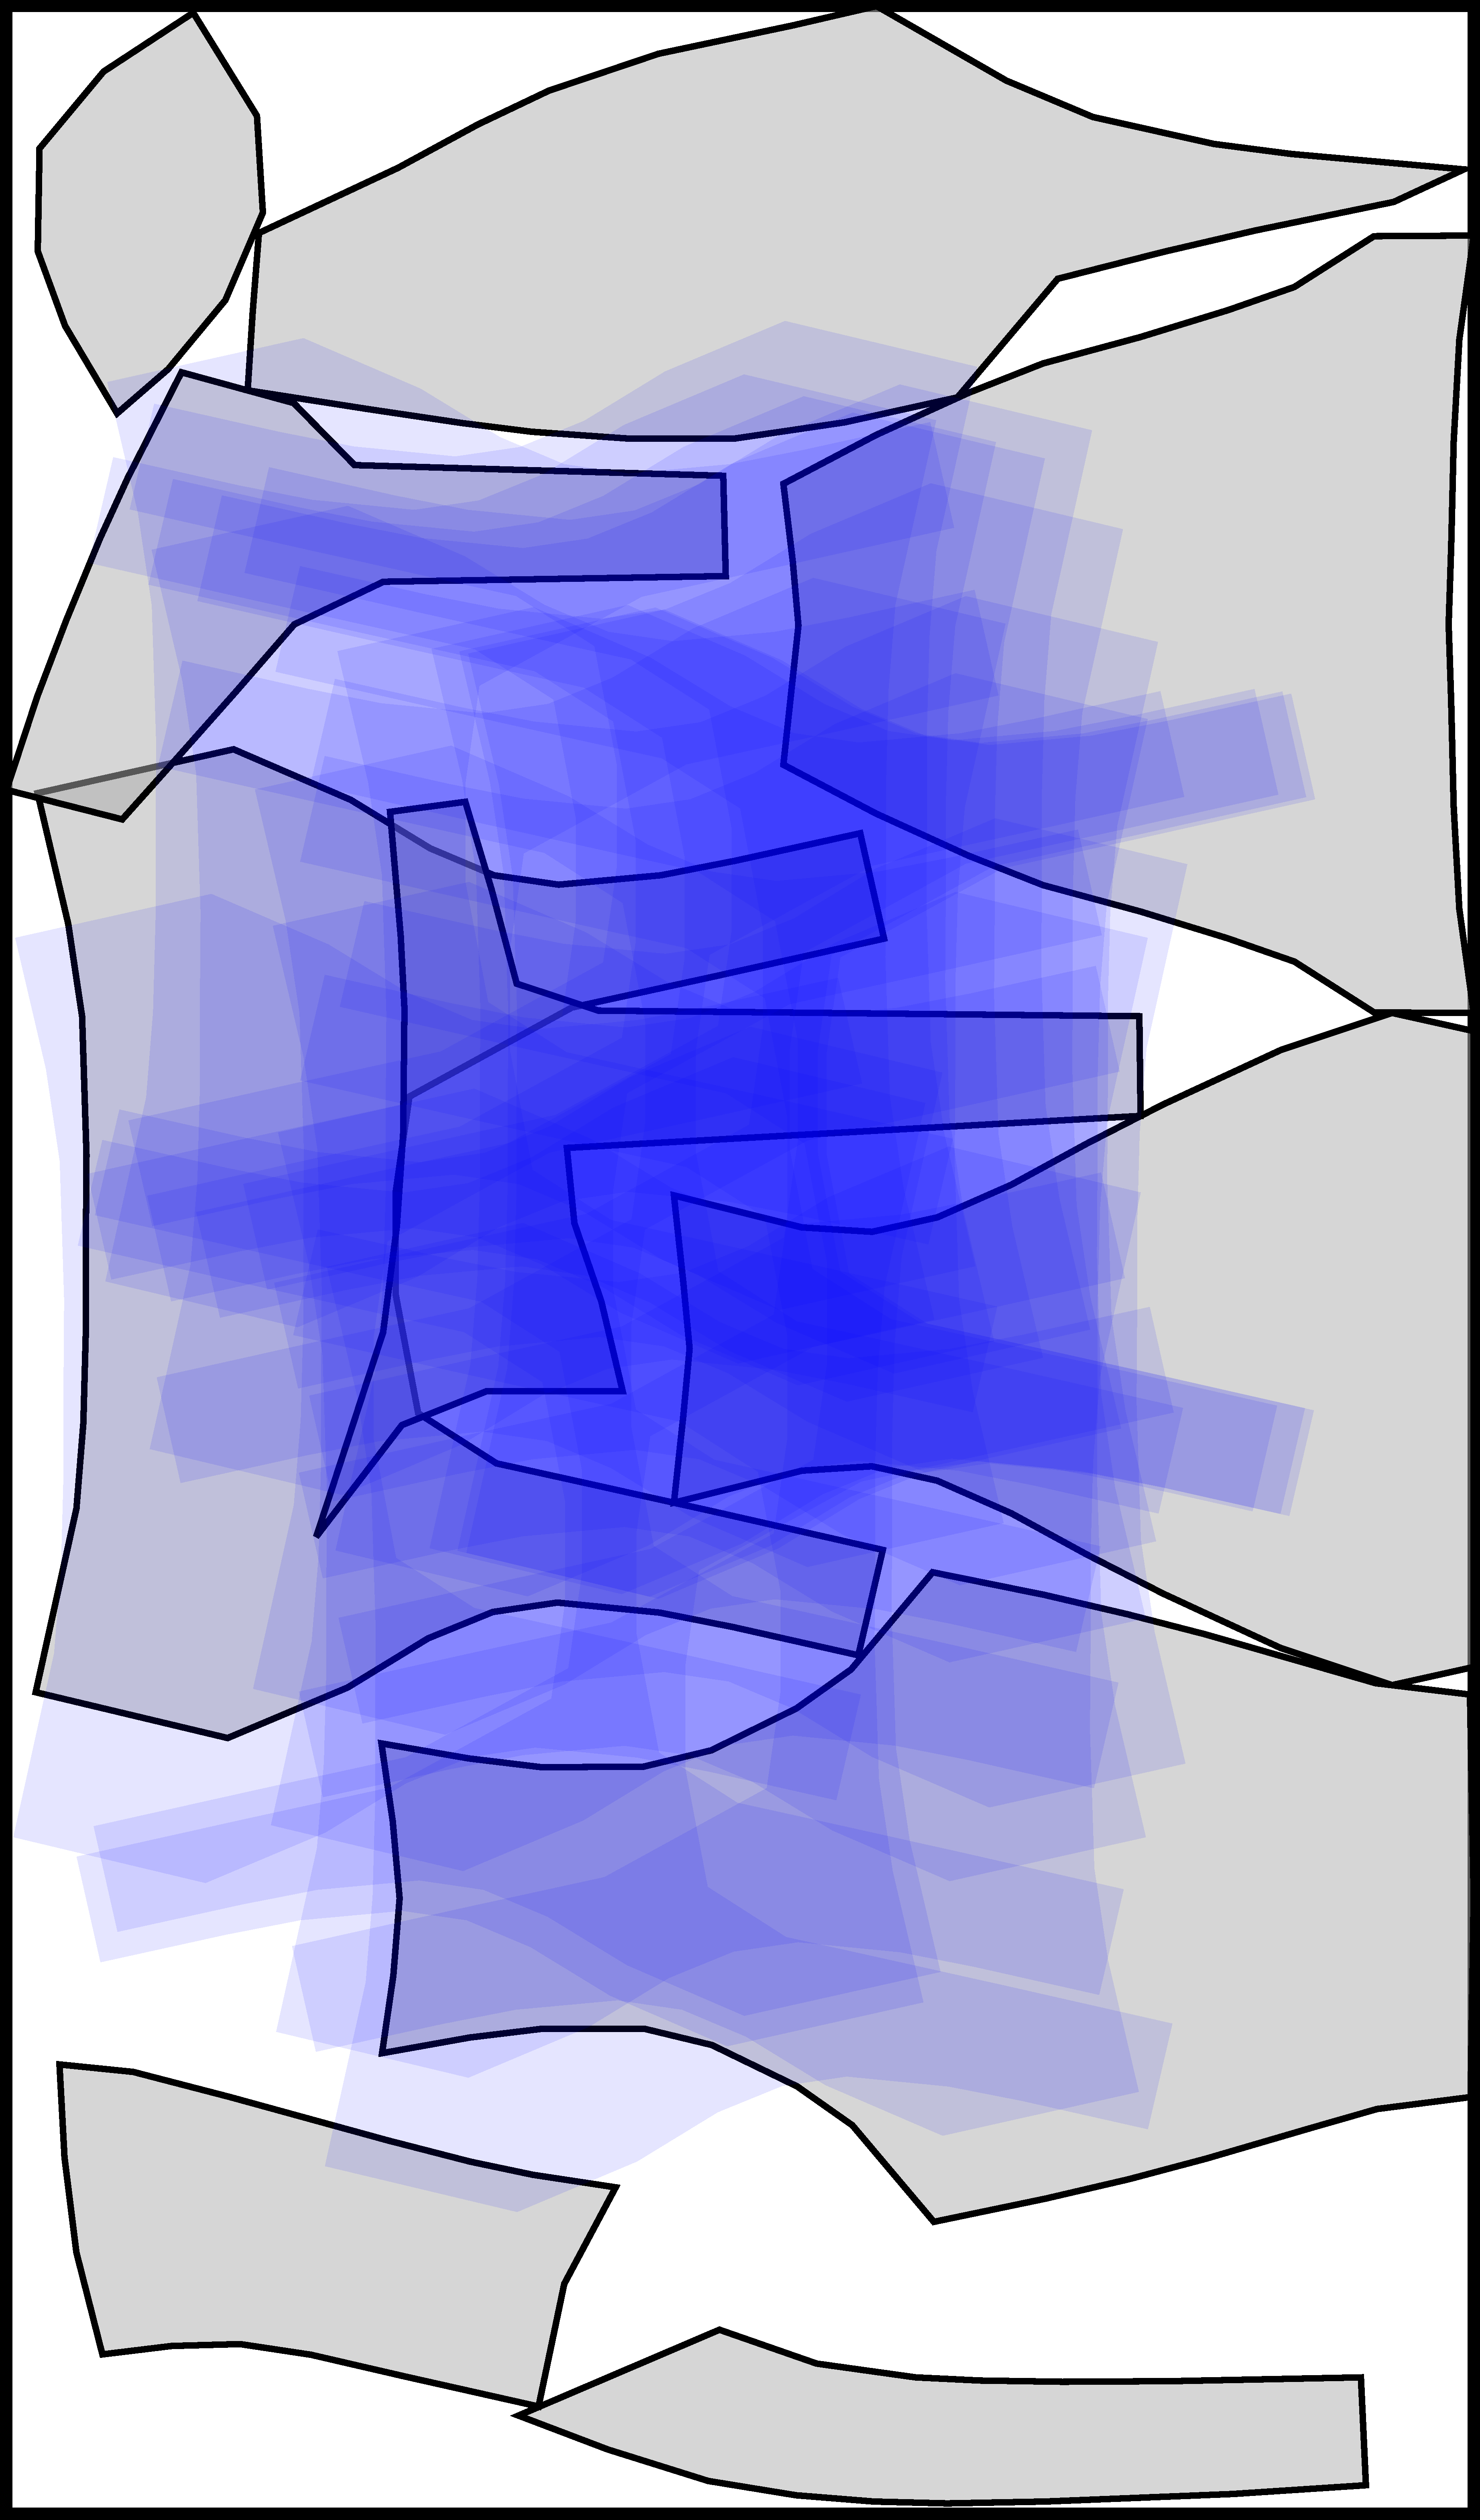
\includegraphics[height=\subfigheight]{samples_1184_2_svg-tex.pdf}
        \caption{Random samples near the current position: $T_{foc}$}
        \label{fig:sampling_loc}
    \end{subfigure}
    \begin{subfigure}[t]{.19\textwidth}
        \centering
        %\includesvg[height=\subfigheight]{samples/inverted/samples_1184_3.svg}
        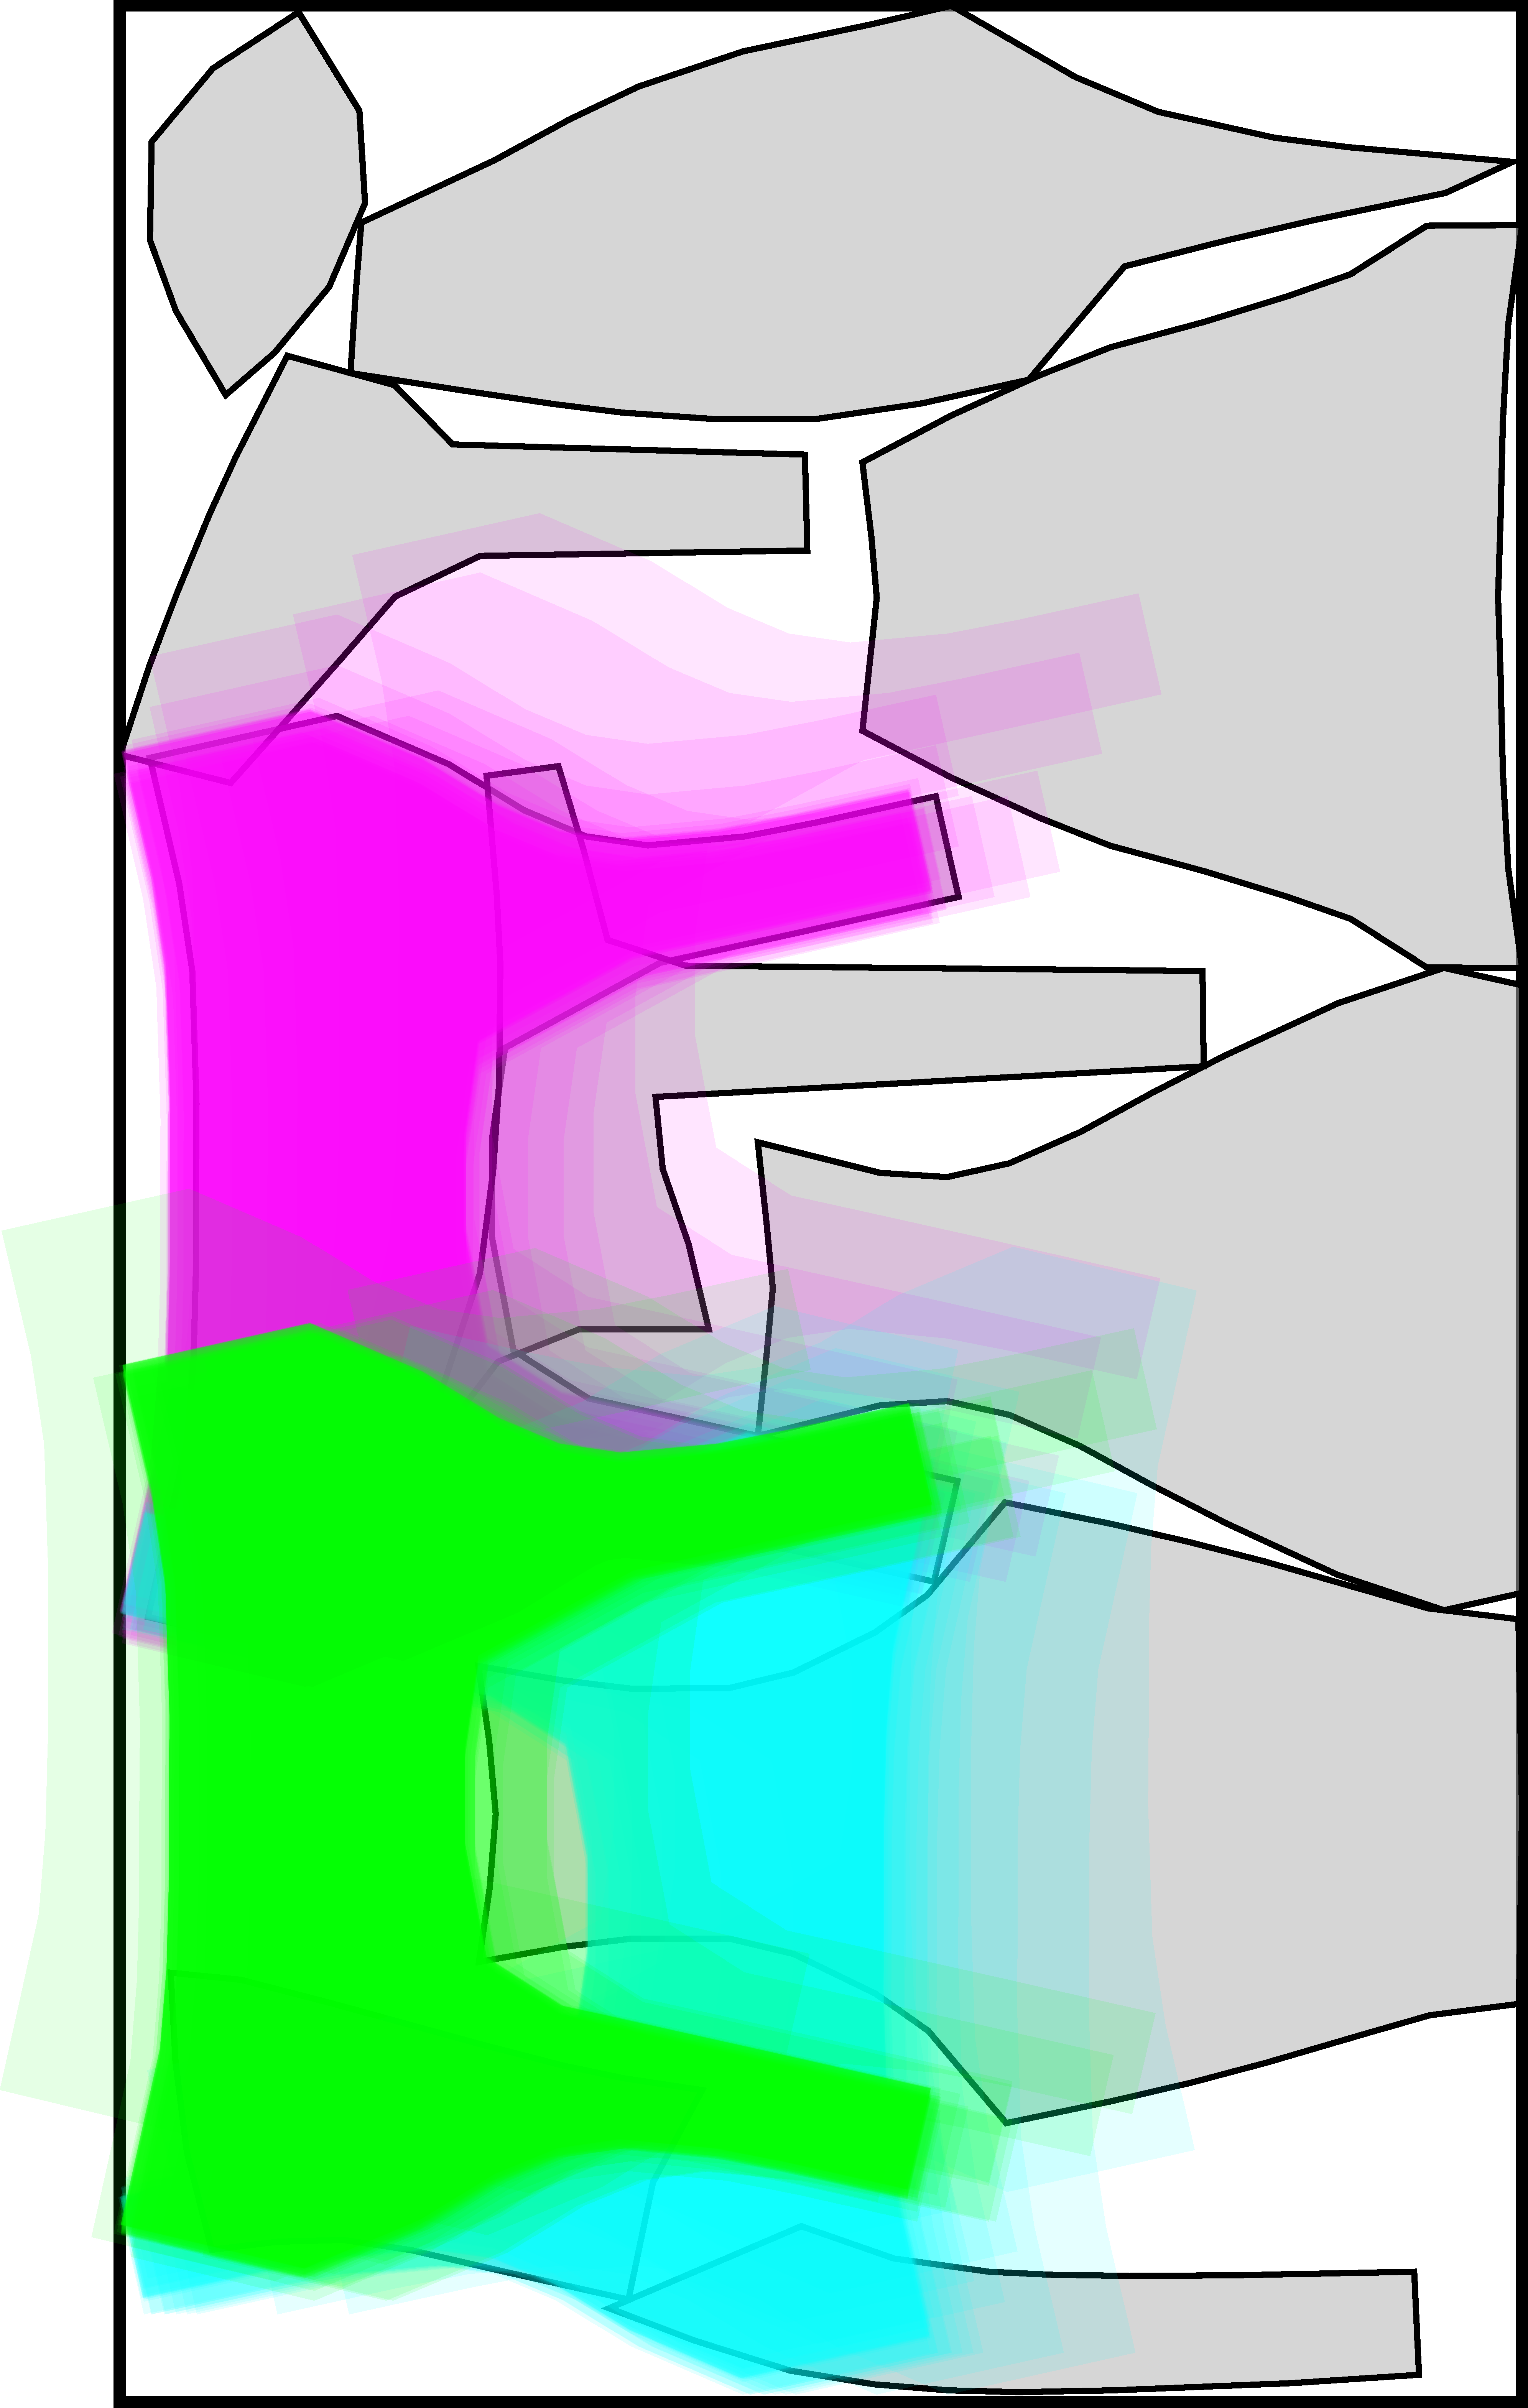
\includegraphics[height=\subfigheight]{samples_1184_3_svg-tex.pdf}
        \caption{Refinement \\ of 3 samples}
        \label{fig:sampling_cd}
    \end{subfigure}
    \begin{subfigure}[t]{.19\textwidth}
        \centering
        %\includesvg[height=\subfigheight]{samples/inverted/samples_1185.svg}
        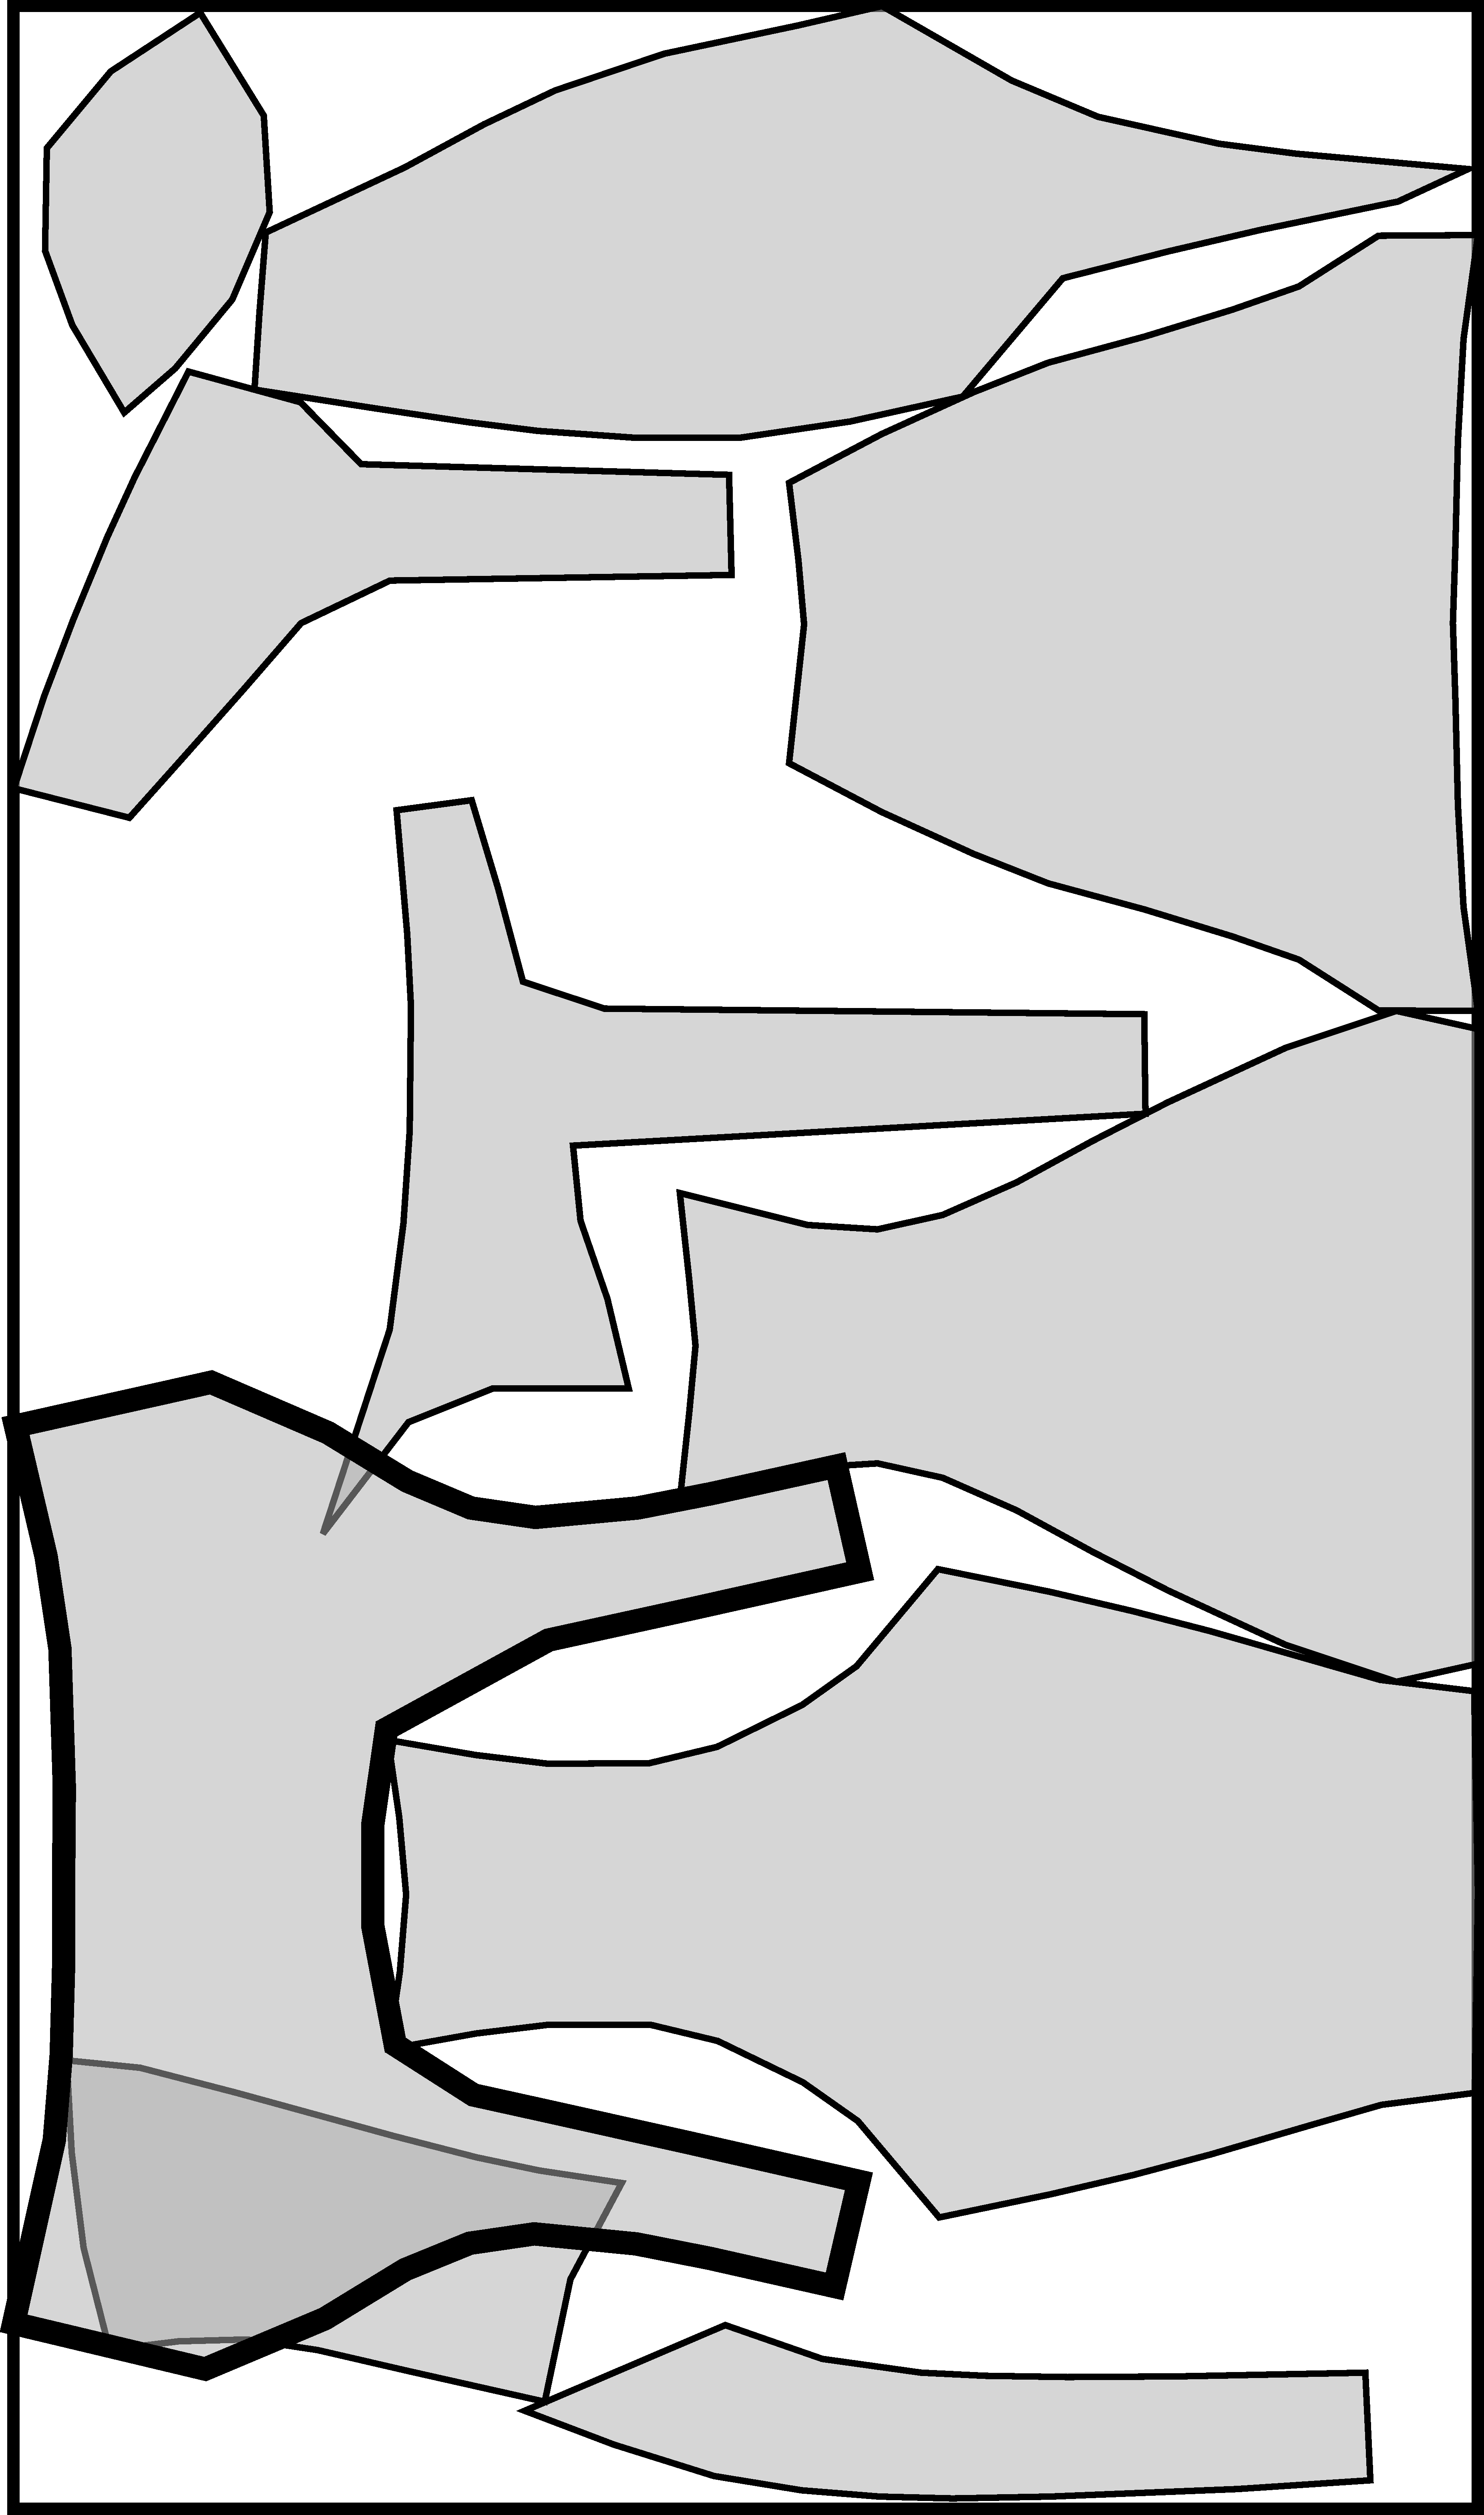
\includegraphics[height=\subfigheight]{samples_1185_svg-tex.pdf}
        \caption{After}
        \label{fig:sampling_after}
    \end{subfigure}
    \caption{Searching for a new position for a single item (in bold) using the \texttt{perform\_sampling} procedure.}
    \label{fig:sampling}
\end{figure}